\documentclass{mm2}
\usepackage{bbm}
\usepackage{bbold}

\newcommand{\pdiff}[2]{\frac{\partial #1}{\partial #2}}
\newcommand{\pddiff}[2]{\frac{\partial^2 #1}{\partial #2^2}}


\cisid{xabc123} % retplace with your own
\title{Your Title}
\begin{document}

\begin{abstract}
  Your Abstract.
\end{abstract}



\section{Introduction}
Your Introduction

\section{A section}

Example of an equation
\begin{eqnarray}
\Delta I_i &=& K S_i I_i/N \nonumber\\
S_{i+1} &=& S_i  - \Delta I_i \nonumber\\
I_{i+1} &=& I_i  + \Delta I_i.
\label{eq:simpSE}
\end{eqnarray}

We can refer to that equation using (\ref{eq:simpSE})

\vspace{5mm}
\begin{answer}{1}
  This will be you answer to problem 1, but move this where appropriate.
\end{answer}

You should also add some text outside the answer to questions of course.

\vspace{5mm}
\begin{answer}{3}
  This will be you answer to problem 3, but move this where appropriate.
\end{answer}

The questions do not need to be answered in the numerical order.

\vspace{5mm}
\begin{answer}{2}
  This will be you answer to problem 2, but move this where appropriate.
\end{answer}

Then there will probably be more text here split over a number of lines or
equations or whatever.

\begin{answer}{4}
  This will be you answer to problem 4, but move this where appropriate.
\end{answer}


This is how we include a figure
\begin{figure}[ht!]
  \centering
  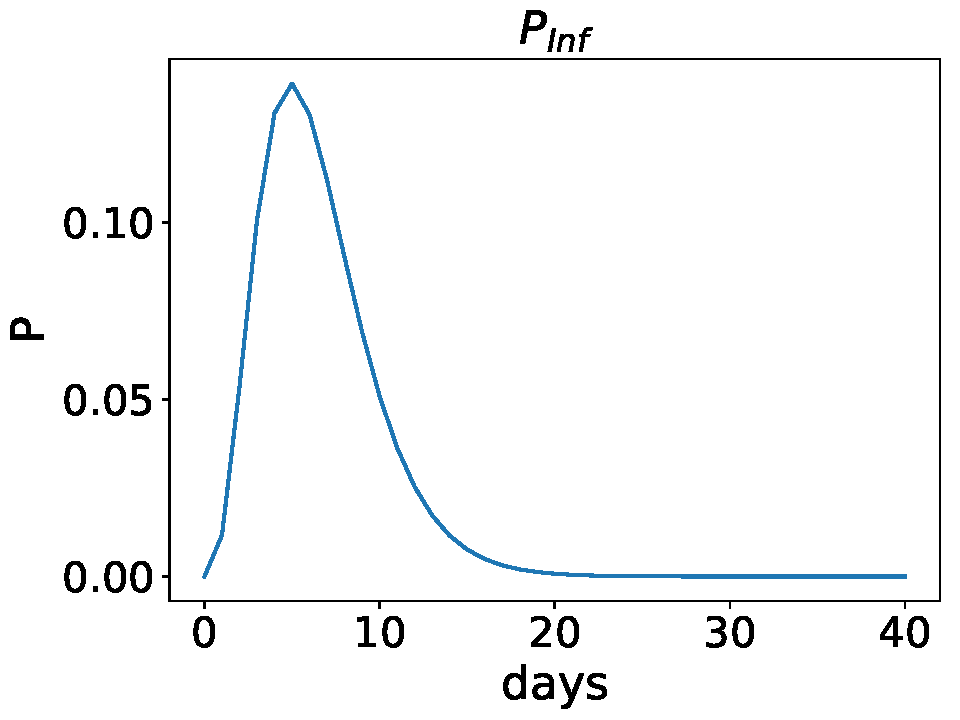
\includegraphics[width=60mm]{Pi.pdf}
  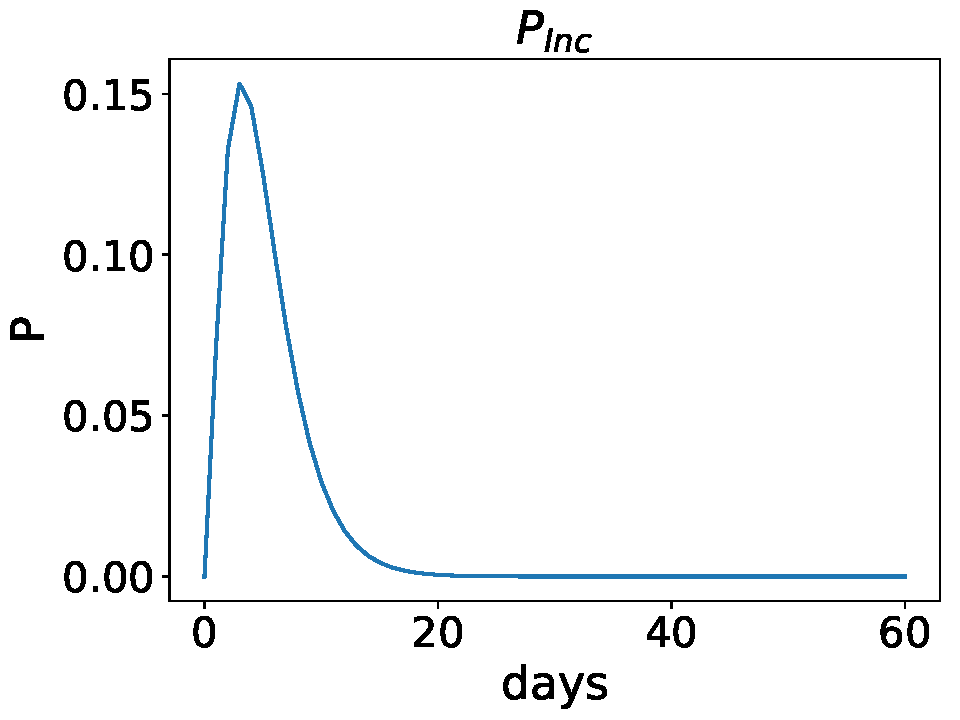
\includegraphics[width=60mm]{Pinc.pdf}\\
  \hspace{5mm}(a) \hspace{55mm} (b)\\
\caption{Probability distributions: a) Infectiousness after infection b) Showing symptoms after infection
\label{fig:probs}}
\end{figure}

\vspace{5mm}
\begin{answer}{5}
  This will be you answer to problem 5, but move this where appropriate.
\end{answer}

In figure \ref{fig:probs} we can't see anything interesting yet.
An appropriate figure is needed!

\vspace{5mm}
\begin{answer}{6}
  This will be you answer to problem 6, but move this where appropriate.
\end{answer}

All your references should be cited. You can do this as follows
: It has been shown that \cite{Imperial2020} all is well and also
that\cite{Lauer2020} we can nevertheless hope for a better future.



\section{Conclusions}
Your conclusions

The references: do you have any others.

\begin{thebibliography}{99}
\bibitem{Imperial2020}
Flaxman {\it et. al},
{\it Report 13: ­­Estimating the number of infections and the impact of non-pharmaceutical interventions on COVID-19 in 11 European countries}
\href{https://www.imperial.ac.uk/mrc-global-infectious-disease-analysis/covid-19/}{https://www.imperial.ac.uk/mrc-global-infectious-disease-analysis/covid-19/}

\bibitem{Lauer2020}
  Stephen A. Lauer {\it et. al},
{\it The Incubation Period of Coronavirus Disease 2019 (COVID-19) From
Publicly Reported Confirmed Cases: Estimation and Application}
Ann. Intern. Med. doi:10.7326/M20-0504




\bibliographystyle{plain}
\end{thebibliography}{}
\end{document}
